\documentclass[aspectratio=169]{beamer}

% ----- Theme & Colors -----
\usetheme{Madrid}
\usecolortheme{default}
\definecolor{primary}{RGB}{20,60,120}       % deep navy
\definecolor{accent}{RGB}{0,120,180}        % teal-blue
\definecolor{serverblue}{HTML}{1F4E79}
\definecolor{clientgreen}{HTML}{2E7D32}
\definecolor{accentorange}{HTML}{C75B12}
\definecolor{softgray}{HTML}{F5F7FA}

\setbeamercolor{palette primary}{bg=primary,fg=white}
\setbeamercolor{palette secondary}{bg=accent,fg=white}
\setbeamercolor{palette tertiary}{bg=primary!80,fg=white}
\setbeamercolor{title}{bg=primary,fg=white}
\setbeamercolor{frametitle}{bg=primary,fg=white}
\setbeamercolor{item}{fg=accent}
\setbeamercolor{block title}{bg=primary,fg=white}
\setbeamercolor{block body}{bg=blue!4,fg=black}
\setbeamercolor{block title example}{bg=clientgreen!90,fg=white}
\setbeamercolor{block body example}{bg=green!4,fg=black}
\setbeamercolor{block title alert}{bg=accentorange!90,fg=white}
\setbeamercolor{block body alert}{bg=orange!4,fg=black}

% ----- Packages -----
\usepackage[utf8]{inputenc}
\usepackage[T1]{fontenc}
\usepackage{amsmath,amssymb}
\usepackage{graphicx}
\usepackage{tikz}
\usetikzlibrary{arrows.meta, positioning, shapes.geometric, calc}
\usepackage{booktabs}
\usepackage{tabularx}

% ----- Title Page Info -----
\title[Federated Learning: FedAvg vs FedProx in Agriculture]{Evaluating FedAvg and FedProx for Federated Crop Disease Detection under Data Heterogeneity}
\subtitle{A Simulated Collaborative Agricultural Network with Non-IID Foliar Distributions}
\author[Dario Pomasqui]{Dario Pomasqui}
\institute[Yachay Tech]{School of Mathematical and Computational Sciences\\Distributed Systems, Machine Learning \& Precision Agriculture\\Yachay Tech University}
\date{\today}

\begin{document}

% =====================================================================
% Slide 1: Title
% =====================================================================
\begin{frame}
    \titlepage
\end{frame}

% =====================================================================
% Slide 2: Real-World Motivation: Agriculture & Distributed Realities
% =====================================================================
\begin{frame}{Real-World Motivation: Agricultural Impact \& Data Silos}
    \textbf{The Agronomic and Global Food Security Context:}
    \begin{itemize}
        \item Crop foliar diseases account for \textbf{20\% to 40\% annual yield reduction} across staple crops worldwide (Savary et al., \textit{Nat. Ecol. Evol.}, 2019).
        \item Early computer vision diagnosis can \textbf{cut chemical pesticide misuse by up to 50\%} (FAO, 2022).
    \end{itemize}
    \vspace{0.12cm}
    \textbf{Why Centralized Machine Learning Fails in Agricultural Reality:}
    \begin{columns}[T]
        \begin{column}{0.48\textwidth}
            \begin{block}{Commercial Confidentiality \& Sovereignty}
                Photographic records of crop health, infestations, and yield are sensitive trade secrets; producers resist cloud exposure.
            \end{block}
        \end{column}
        \begin{column}{0.48\textwidth}
            \begin{block}{Rural WAN Bandwidth Bottlenecks}
                Farms operate over constrained cellular/satellite uplinks; transmitting gigabytes of high-res foliar photography is unfeasible.
            \end{block}
        \end{column}
    \end{columns}
    \vspace{0.12cm}
    {\small \textbf{The Distributed Paradigm:} \textbf{Federated Learning (FL)} enables decentralized collaborative training where raw foliar images remain on-premises and only numerical model parameters circulate.}
\end{frame}

% =====================================================================
% Slide 3: The Distributed Systems Challenge: Non-IID & Client Drift
% =====================================================================
\begin{frame}{The Distributed Challenge: Non-IID Foliar Skew \& Client Drift}
    \textbf{Agricultural Data is Intrinsically Non-IID (Statistical Heterogeneity):}
    \begin{columns}[T]
        \begin{column}{0.31\textwidth}
            \begin{exampleblock}{Farm A (Humid Valley)}
                \textbf{Dominant:} Necrotic Blights (Rust, Early/Late Blight).\\
                \textit{Negligible bacterial spots.}
            \end{exampleblock}
        \end{column}
        \begin{column}{0.31\textwidth}
            \begin{exampleblock}{Farm B (Highland Zone)}
                \textbf{Dominant:} Bacterial Pathologies (Bacterial Spot, Mold).\\
                \textit{Negligible fungal blights.}
            \end{exampleblock}
        \end{column}
        \begin{column}{0.31\textwidth}
            \begin{exampleblock}{Farm C (Lowland Fields)}
                \textbf{Dominant:} Viral Infections \& Healthy Foliage.\\
                \textit{Negligible necrotic blights.}
            \end{exampleblock}
        \end{column}
    \end{columns}
    \vspace{0.12cm}
    \textbf{Sensor and Covariate Shift:} Ambient solar illumination, soil backgrounds, and smartphone optics.
    \vspace{0.12cm}
    \begin{alertblock}{The Distributed Systems Consequence: Client Drift}
        Local gradient updates steer parameters toward local optima that conflict with the global objective. Standard \textbf{FedAvg} exhibits severe round-to-round oscillation, slow convergence, and \textbf{catastrophic accuracy degradation on minority disease classes}.
    \end{alertblock}
\end{frame}

% =====================================================================
% Slide 4: Research Question & Formal Hypotheses
% =====================================================================
\begin{frame}{Research Question \& Formal Hypotheses}
    \begin{center}
        \normalsize
        \textit{"To what extent does \textbf{FedProx} improve diagnostic performance, consensus stability, and cross-client generalization compared to \textbf{FedAvg} in a distributed plant disease detection system when three farm nodes possess statistically heterogeneous (non-IID) data distributions?"}
    \end{center}
    \vspace{0.15cm}
    \begin{columns}[T]
        \begin{column}{0.48\textwidth}
            \begin{block}{Hypothesis 1 (Performance Equity)}
                \footnotesize Under IID data, FedAvg and FedProx achieve parity; under acute non-IID skew, FedProx achieves superior macro-F1 and preserves minority class recall.
            \end{block}
            \begin{block}{Hypothesis 2 (Optimization Stability)}
                \footnotesize FedProx dampens inter-round oscillations via its proximal anchor, yielding lower inter-round variance $S_{\Delta acc}$.
            \end{block}
        \end{column}
        \begin{column}{0.48\textwidth}
            \begin{block}{Hypothesis 3 (Parameter Sensitivity)}
                \footnotesize An intermediate proximal penalty ($\mu \in [0.01, 0.1]$) balances consensus stability vs.\ optimization stalling ($\mu \ge 1.0$).
            \end{block}
            \begin{block}{Hypothesis 4 (Fault Tolerance under Dropout)}
                \footnotesize When a node disconnects (round $t=5$), FedProx retains higher parameter stability and diagnostic resilience.
            \end{block}
        \end{column}
    \end{columns}
\end{frame}

% =====================================================================
% Slide 5: Distributed Systems Foundations & Algorithmic Consensus
% =====================================================================
\begin{frame}{Distributed Foundations: Protocols \& Optimization}
    \begin{columns}[T]
        \begin{column}{0.49\textwidth}
            \textbf{Distributed Coordination Principles:}
            \begin{itemize}\footnotesize
                \item \textbf{Star Topology \& RPC:} Coordinator orchestrates workers via gRPC messages (\texttt{FitIns}, \texttt{FitRes}).
                \item \textbf{Barrier Latency Model:}
                {\scriptsize
                \[
                T_{\text{round}}^{(t)} = \max_{k \in \mathcal{K}_t} \{T_{\text{down}}^{(k)} + T_{\text{comp}}^{(k)} + T_{\text{up}}^{(k)}\} + T_{\text{agg}}
                \]}
                \item \textbf{Communication Complexity:} Exchanging serialized weights ($B_{\text{round}} = 8Kd$ bytes) reduces network payload by \textbf{$>98\%$} vs.\ raw image transmission.
            \end{itemize}
        \end{column}
        \begin{column}{0.49\textwidth}
            \textbf{Mathematical Optimization Formulation:}
            \begin{itemize}\footnotesize
                \item \textbf{Baseline: FedAvg (McMahan et al., 2017)}
                {\scriptsize
                \[
                w^{(t+1)} = \sum_{k=1}^K \frac{n_k}{n} w_k^{(t+1)}
                \]}
                \item \textbf{Investigated: FedProx (Li et al., 2020)}
                {\scriptsize
                \[
                \min_{w} F_k(w) + \frac{\mu}{2}\left\| w - w^{(t)} \right\|_2^2
                \]}
                Elastic proximal penalty pulls divergent worker gradients toward global centroid.
            \end{itemize}
        \end{column}
    \end{columns}
\end{frame}

% =====================================================================
% Slide 6: Understanding the Barrier Latency Formula
% =====================================================================
\begin{frame}{Understanding the Barrier Latency Formula}
    \begin{center}
        \textbf{Barrier Latency Model --- Round Completion Time:}
        \vspace{0.3cm}

        \[
        T_{\text{round}}^{(t)}
        =
        \max_{k\in \mathcal{K}_t}
        \left\{
        T_{\text{down}}^{(k)}
        +T_{\text{comp}}^{(k)}
        +T_{\text{up}}^{(k)}
        \right\}
        +T_{\text{agg}}
        \]
    \end{center}
    \vspace{0.2cm}
    \textbf{Each symbol represents the following:}
    \vspace{0.15cm}

    \begin{center}
    \footnotesize
    \renewcommand{\arraystretch}{1.35}
    \begin{tabular}{@{} >{\centering\arraybackslash}p{3.2cm} p{9.5cm} @{}}
        \toprule
        \textbf{Symbol} & \textbf{Meaning} \\
        \midrule
        $T_{\text{round}}^{(t)}$   & Total time of round $t$ (from broadcast to aggregation completion). \\
        $\mathcal{K}_t$            & Set of participating clients in that round. \\
        $T_{\text{down}}^{(k)}$    & Time for client $k$ to \textbf{receive} (download) the global model. \\
        $T_{\text{comp}}^{(k)}$    & Time for client $k$ to \textbf{train locally} ($E$ SGD epochs). \\
        $T_{\text{up}}^{(k)}$      & Time for client $k$ to \textbf{upload} its updated parameters to the server. \\
        $T_{\text{agg}}$           & Time the server needs to \textbf{aggregate} (combine) all client updates. \\
        $\max$                     & Selects the \textbf{slowest client} --- the round cannot advance until every participant finishes. \\
        \bottomrule
    \end{tabular}
    \end{center}
    \vspace{0.15cm}
    \footnotesize \textbf{Key insight:} The barrier synchronization model means the \textit{slowest} node (straggler) dictates the round duration. This is why client heterogeneity directly impacts system throughput.
\end{frame}

% =====================================================================
% Slide 7: Farm Nodes as Distributed Compute Nodes
% =====================================================================
\begin{frame}{Farm Nodes as Distributed Compute Nodes}
    {\small \textbf{Shared-Nothing Architecture:} Each farm is an autonomous node with private storage, independent compute, and an isolated model replica. No shared memory or filesystem --- communication exclusively via serialized message passing.}
    \vspace{0.1cm}
    \begin{columns}[T]
        \begin{column}{0.49\textwidth}
            \begin{block}{Node Properties}
                \begin{itemize}\footnotesize
                    \item \textbf{Local State Isolation:} Node $k$ maintains private state $\sigma_k = (w_k, \mathcal{D}_k, n_k, t_k)$. No other node can read or modify it.
                    \item \textbf{Independent Failure Domain:} Crash at Farm~A does not propagate to B or C --- \textit{failure isolation} across fault domains.
                    \item \textbf{Stateless Interactions:} Each \texttt{FitIns}/\texttt{FitRes} is self-contained --- enables transparent node replacement.
                \end{itemize}
            \end{block}
        \end{column}
        \begin{column}{0.49\textwidth}
            \begin{block}{Scalability \& Consensus}
                \begin{itemize}\footnotesize
                    \item \textbf{Horizontal Scalability:} Adding node $K{+}1$ requires only $\mathcal{O}(Kd)$ additional aggregation cost --- no data repartitioning.
                    \item \textbf{Relaxed State Replication:} Unlike Paxos/Raft, federated consensus permits optimistic local execution + post-hoc reconciliation.
                    \item \textbf{Aggregation as Consensus:} $w^{(t+1)} = \sum_k \frac{n_k}{n} w_k^{(t+1)}$ merges divergent replicas into global state.
                \end{itemize}
            \end{block}
        \end{column}
    \end{columns}
\end{frame}

% =====================================================================
% Slide 8: Node Lifecycle & Distributed Fault Scenarios
% =====================================================================
\begin{frame}{Node Lifecycle \& Distributed Fault Scenarios}
    \begin{columns}[T]
        \begin{column}{0.50\textwidth}
            \textbf{Node State Machine (per Farm):}
            \vspace{0.1cm}
            \begin{enumerate}
                \item \textbf{IDLE} --- Awaiting \texttt{FitIns} RPC.
                \item \textbf{SYNCHRONIZING} --- Deserializing $w^{(t)}$; overwriting local replica.
                \item \textbf{TRAINING} --- Executing $E$ local SGD epochs; state \textit{diverges} from global.
                \item \textbf{REPORTING} --- Serializing $w_k^{(t+1)}$ into \texttt{FitRes}; uploading to coordinator.
                \item \textbf{PARTITIONED} --- Network loss or crash detected via timeout $\tau_{\text{timeout}}$; node excluded from quorum $\mathcal{S}_t$.
            \end{enumerate}
            \vspace{0.1cm}
            \footnotesize \textbf{Recovery:} Partitioned node re-joins by receiving next round's $w^{(t+1)}$ --- \textit{state catch-up} via parameter overwrite.
        \end{column}
        \begin{column}{0.48\textwidth}
            \textbf{Fault Tolerance Mechanisms:}
            \begin{itemize}
                \item \textbf{Network Partitions:} Timeout $\tau_{\text{timeout}}$ distinguishes straggler vs.\ unreachable node.
                \item \textbf{Quorum-Based Aggregation:}
                {\footnotesize
                \[
                w^{(t+1)} = \sum_{k \in \mathcal{S}_t} \frac{n_k}{\sum_{j \in \mathcal{S}_t} n_j} w_k^{(t+1)}
                \]
                }
                \item \textbf{Majority Quorum:} $|\mathcal{S}_t| \geq \lceil K/2 \rceil + 1$ prevents split-brain divergence.
                \item \textbf{Byzantine Awareness:} Crash-stop model assumed; Krum/trimmed-mean aggregation supports $f < K/3$ malicious nodes (future work).
            \end{itemize}
        \end{column}
    \end{columns}
\end{frame}

% =====================================================================
% Slide 9: Collaborative Farm Network Architecture
% =====================================================================
\begin{frame}{Collaborative Farm Network Architecture}
    \begin{center}
    \resizebox{0.92\textwidth}{!}{%
    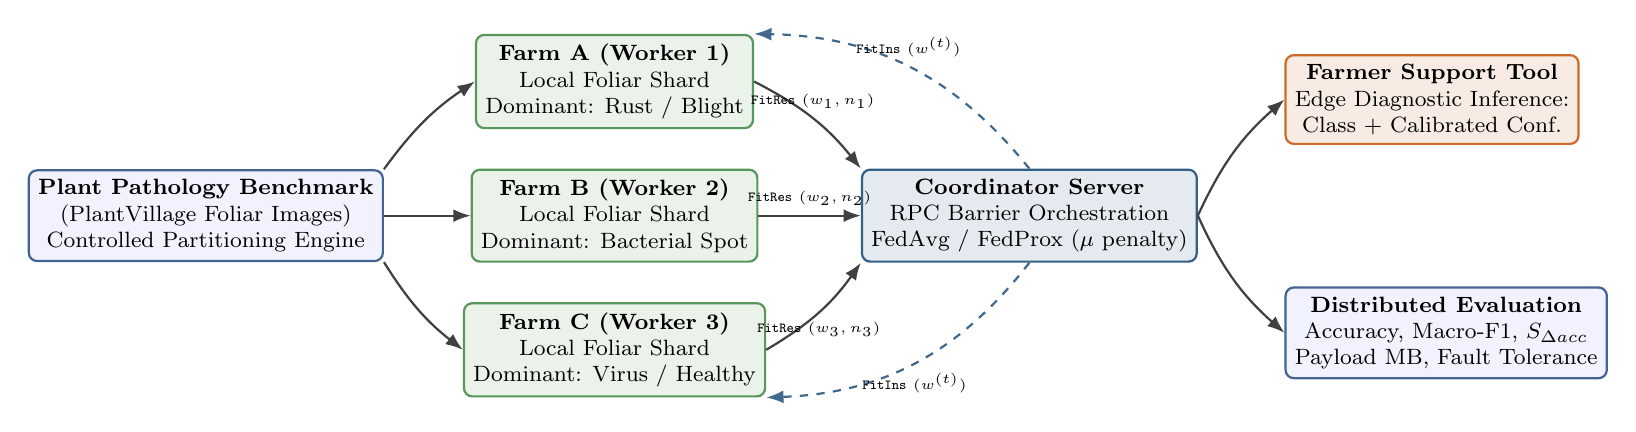
\begin{tikzpicture}[
        font=\footnotesize,
        node distance=0.8cm and 1.2cm,
        block/.style={draw=primary!80, thick, fill=blue!5, rounded corners=3pt, align=center, minimum width=2.4cm, minimum height=0.85cm},
        client/.style={draw=clientgreen!80, thick, fill=clientgreen!10, rounded corners=3pt, align=center, minimum width=2.6cm, minimum height=0.85cm},
        server/.style={draw=serverblue!90, thick, fill=serverblue!12, rounded corners=3pt, align=center, minimum width=3.2cm, minimum height=1.0cm},
        app/.style={draw=accentorange!90, thick, fill=accentorange!12, rounded corners=3pt, align=center, minimum width=2.8cm, minimum height=0.9cm},
        arrow/.style={-{Latex[length=2.2mm]}, thick, draw=black!75},
        update/.style={-{Latex[length=2.2mm]}, thick, dashed, draw=serverblue!85}
    ]
    % Data Source
    \node[block] (data) {\textbf{Plant Pathology Benchmark}\\(PlantVillage Foliar Images)\\Controlled Partitioning Engine};

    % Clients
    \node[client, right=1.1cm of data] (c2) {\textbf{Farm B (Worker 2)}\\Local Foliar Shard\\Dominant: Bacterial Spot};
    \node[client, above=0.5cm of c2] (c1) {\textbf{Farm A (Worker 1)}\\Local Foliar Shard\\Dominant: Rust / Blight};
    \node[client, below=0.5cm of c2] (c3) {\textbf{Farm C (Worker 3)}\\Local Foliar Shard\\Dominant: Virus / Healthy};

    % Server
    \node[server, right=1.3cm of c2] (server) {\textbf{Coordinator Server}\\RPC Barrier Orchestration\\FedAvg / FedProx ($\mu$ penalty)};

    % App & Evaluation
    \node[app, above right=0.3cm and 1.1cm of server] (app) {\textbf{Farmer Support Tool}\\Edge Diagnostic Inference:\\Class + Calibrated Conf.};
    \node[block, below right=0.3cm and 1.1cm of server] (eval) {\textbf{Distributed Evaluation}\\Accuracy, Macro-F1, $S_{\Delta acc}$\\Payload MB, Fault Tolerance};

    % Connections
    \draw[arrow] (data.north east) to[bend left=10] (c1.west);
    \draw[arrow] (data.east) -- (c2.west);
    \draw[arrow] (data.south east) to[bend right=10] (c3.west);

    \draw[arrow] (c1.east) to[bend left=12] node[above, font=\tiny] {\texttt{FitRes} ($w_1, n_1$)} (server.north west);
    \draw[arrow] (c2.east) -- node[above, font=\tiny] {\texttt{FitRes} ($w_2, n_2$)} (server.west);
    \draw[arrow] (c3.east) to[bend right=12] node[below, font=\tiny] {\texttt{FitRes} ($w_3, n_3$)} (server.south west);

    \draw[update] (server.north) to[bend right=25] node[above, font=\tiny] {\texttt{FitIns} ($w^{(t)}$)} (c1.north east);
    \draw[update] (server.south) to[bend left=25] node[below, font=\tiny] {\texttt{FitIns} ($w^{(t)}$)} (c3.south east);

    \draw[arrow] (server.east) to[bend left=12] (app.west);
    \draw[arrow] (server.east) to[bend right=12] (eval.west);

    \end{tikzpicture}
    }
    \end{center}
    \vspace{0.1cm}
    \footnotesize \textbf{Distributed Decoupling:} Private photographs never leave local worker boundaries; only serialized parameter tensors and sample counts cross the network channels.
\end{frame}

% =====================================================================
% Slide 10: Controlled Non-IID Partitioning & Edge Calibration
% =====================================================================
\begin{frame}{Controlled Non-IID Partitioning \& Edge Support Tool}
    \begin{columns}[T]
        \begin{column}{0.52\textwidth}
            \textbf{Four Rigorous Partitioning Regimes:}
            \begin{enumerate}
                \item \textbf{IID Baseline ($\alpha \to \infty$):} Balanced uniform distribution ($n_k = N/3, \mathbf{p}_k \approx \mathbf{p}_0$).
                \item \textbf{Low Non-IID ($\alpha = 1.0$):} Dirichlet distribution with mild sample variations.
                \item \textbf{Medium Non-IID ($\alpha = 0.5$):} Dirichlet distribution with moderate class concentration ($<10\%$ in minority classes).
                \item \textbf{High Non-IID ($85/15$ Disjoint Rule):} Extreme geographic skew where each farm receives 85\% of an exclusive disease cluster and 7.5\% from others.
            \end{enumerate}
        \end{column}
        \begin{column}{0.46\textwidth}
            \textbf{Farmer Support Tool \& Calibration:}
            \begin{itemize}
                \item \textbf{Edge Input:} Technician captures foliar photo in field.
                \item \textbf{Model Inference:} Local feedforward pass on compiled global model.
                \item \textbf{Confidence Calibration:} Standard softmax is overconfident (Guo et al., 2017); evaluated via post-hoc \textbf{Temperature Scaling} and \textbf{Expected Calibration Error (ECE)}.
                \item \textbf{Agronomic Advisory:} Specific treatment guidance (fungicide, isolation, monitoring).
            \end{itemize}
        \end{column}
    \end{columns}
\end{frame}

% =====================================================================
% Slide 11: Targeted Experimental Matrix (6 Key Tracks)
% =====================================================================
\begin{frame}{Targeted Experimental Matrix (6 Systematic Tracks)}
    \begin{columns}[T]
        \begin{column}{0.48\textwidth}
            \begin{block}{1. FedAvg vs. FedProx Optimization}
                \footnotesize Compares global diagnostic accuracy, loss trajectories, and convergence speed across rounds.
            \end{block}
            \vspace{0.1cm}
            \begin{block}{2. Statistical Heterogeneity Impact}
                \footnotesize Quantifies accuracy penalty across $\alpha \in \{\infty, 1.0, 0.5, \text{disjoint}\}$ as cross-farm skew intensifies.
            \end{block}
            \vspace{0.1cm}
            \begin{block}{3. Proximal Parameter Sweep}
                \footnotesize Evaluates $\mu \in \{0.001, 0.01, 0.1, 1.0\}$ to detect optimal balance vs.\ local update stalling.
            \end{block}
        \end{column}
        \begin{column}{0.48\textwidth}
            \begin{block}{4. Fault Tolerance \& Node Churn}
                \footnotesize Evaluates system recovery and consensus degradation when Farm C disconnects at round $t=5$.
            \end{block}
            \vspace{0.1cm}
            \begin{block}{5. Communication Complexity}
                \footnotesize Profiles serialized payload (MB/round), barrier completion latency, and rural WAN viability.
            \end{block}
            \vspace{0.1cm}
            \begin{block}{6. Cross-Node \& Minority Equity}
                \footnotesize Assesses per-client test performance and class-wise recall to guarantee equity for small farms.
            \end{block}
        \end{column}
    \end{columns}
    \vspace{0.2cm}
    \centering \footnotesize \textbf{Stability Metric:} $S_{\Delta acc} = \sqrt{\frac{1}{R-1}\sum_{r=2}^R (\Delta acc_r - \overline{\Delta acc})^2}$ (lower indicates smoother optimization).
\end{frame}

% =====================================================================
% Slide 12: Preliminary Results: RabbitMQ Prototype & Quorum Validation
% =====================================================================
\begin{frame}{Preliminary Results: RabbitMQ Prototype \& Quorum Validation}
    \textbf{Empirical Verification of Distributed Coordinator-Worker Prototype:}
    \vspace{0.05cm}
    \begin{center}
    \scriptsize
    \setlength{\tabcolsep}{3.5pt}
    \renewcommand{\arraystretch}{1.2}
    \begin{tabular}{@{} l c c c c p{3.4cm} @{}}
        \toprule
        \textbf{Scenario} & \textbf{Quorum} & \textbf{Samples} & \textbf{Global $w^{(1)}$} & \textbf{Barrier Latency ($T$)} & \textbf{Queue State \& Behavior} \\
        \midrule
        \textbf{Complete Round} & $3/3$ & $N{=}60$ & \textbf{2.8333} & \textbf{120 ms} ($T_{\text{agg}}{=}12.5$\,ms) & Queues drained; manual acks confirmed. \\
        \textbf{Node Dropout} & $2/3$ & $N{=}30$ & \textbf{1.6667} & \textbf{3.00 s} ($\tau$ timeout barrier) & Dynamic re-weighting; C task queued. \\
        \bottomrule
    \end{tabular}
    \end{center}
    \vspace{0.05cm}
    \begin{columns}[T]
        \begin{column}{0.48\textwidth}
            \begin{exampleblock}{Nominal Aggregation ($K=3$)}
                \scriptsize
                \[
                w^{(1)} = \frac{10(1) + 20(2) + 30(4)}{60} = \frac{170}{60} \approx \mathbf{2.8333}
                \]
                \textbf{Barrier Latency:} $T_{\text{barrier}} \approx 120$\,ms; $T_{\text{agg}} = 12.5$\,ms.\\
                Unblocks immediately upon complete quorum.
            \end{exampleblock}
        \end{column}
        \begin{column}{0.48\textwidth}
            \begin{alertblock}{Dropout Resilience ($K=2$, Farm C down)}
                \scriptsize
                \[
                w^{(1)}_{\text{dropout}} = \frac{10(1) + 20(2)}{30} = \frac{50}{30} \approx \mathbf{1.6667}
                \]
                \textbf{Barrier Latency:} $T_{\text{barrier}} = 3.00$\,s (fault detection via $\tau$).\\
                $T_{\text{agg}} = 8.2$\,ms; coordinator advances without deadlock.
            \end{alertblock}
        \end{column}
    \end{columns}
\end{frame}

% =====================================================================
% Slide 13: Distributed Systems Theory Applied to Federated Agriculture
% =====================================================================
\begin{frame}{Distributed Systems Theory in Federated Agriculture}
    \begin{columns}[T]
        \begin{column}{0.48\textwidth}
            \textbf{CAP Theorem Trade-offs (Brewer, 2000):}
            \begin{itemize}
                \item \textbf{Consistency:} All nodes see identical global model.
                \item \textbf{Availability:} Every farm can train locally, even offline.
                \item \textbf{Partition Tolerance:} System survives network failures.
            \end{itemize}
            \vspace{0.15cm}
            \begin{alertblock}{Design Choice: AP System}
                \footnotesize Our federated network prioritizes \textbf{Availability + Partition Tolerance}. Farms train autonomously; coordinator aggregates when reachable. \textbf{Eventual consistency} is achieved over successive communication rounds.
            \end{alertblock}
        \end{column}
        \begin{column}{0.48\textwidth}
            \textbf{Message-Passing \& Logical Clocks:}
            \begin{itemize}
                \item \textbf{RabbitMQ AMQP 0-9-1:} Durable direct/topic exchanges, persistent queues, manual acks (\texttt{FitIns}, \texttt{FitRes}).
                \item \textbf{Causal Ordering ($\prec$):}
                {\footnotesize
                \[
                \text{broadcast} \prec \text{train}_k \prec \text{upload} \prec \text{aggregate}
                \]}
                \item \textbf{Duplicate Suppression:} Monotonic round IDs prevent duplicate uploads from biasing aggregation.
                \item \textbf{Idempotent Aggregation:} Deterministic weighted reduction ensures reproducibility.
            \end{itemize}
        \end{column}
    \end{columns}
\end{frame}

% =====================================================================
% Slide 14: Deliverables \& Academic Architecture Strategy
% =====================================================================
\begin{frame}{Deliverables \& Academic Architecture Strategy}
    \textbf{Software Pipeline \& Modular Separation:}
    \begin{itemize}
        \item \textbf{Distributed Training Simulation:} Implemented in \textbf{Python}, \textbf{PyTorch}, and \textbf{RabbitMQ (AMQP 0-9-1)} for multi-process worker execution, state serialization, and non-IID partitioning.
        \item \textbf{Edge Diagnostic Engine (High-Efficiency C++ Deployment):}
        \begin{itemize}
            \item Trained global CNN exported via \textbf{ONNX} / \textbf{TorchScript}.
            \item Standalone inference runtime using \textbf{ONNX Runtime C++ API} / LibTorch.
            \item Zero Python dependencies on edge device: deploys natively on Raspberry Pi or agricultural field gateways with sub-50ms inference latency.
        \end{itemize}
    \end{itemize}
    \vspace{0.25cm}
    \textbf{Project Deliverables:}
    \begin{itemize}
        \item Reproducible GitHub repository: \url{https://github.com/darioXxx32/IA}.
        \item Automated scripts for partitioning, multi-client simulation, evaluation logs, and visual analytics.
    \end{itemize}
\end{frame}

% =====================================================================
% Slide 15: Project Feasibility, Work Schedule \& Reproducibility
% =====================================================================
\begin{frame}{Project Feasibility, Work Schedule \& Reproducibility}
    \textbf{14-Week Milestone Timeline (Phases 1--6):}
    \vspace{0.05cm}
    \begin{center}
    \tiny
    \renewcommand{\arraystretch}{1.15}
    \begin{tabular}{@{} l p{5.5cm} c l @{}}
        \toprule
        \textbf{Phase} & \textbf{Milestone \& Core Activities} & \textbf{Weeks} & \textbf{Status} \\
        \midrule
        \textbf{Phase 1} & AMQP RabbitMQ Middleware, Quorum \& Unit Tests & W1--3 & \textbf{Completed} \\
        \textbf{Phase 2} & PlantVillage Dirichlet Partitioning ($\alpha \in \{\infty, 1.0, 0.5, \text{disjoint}\}$) & W4--5 & \textbf{Completed} \\
        \textbf{Phase 3} & CNN Architecture \& PyTorch FedAvg/FedProx Loops & W6--7 & \textbf{In Progress} \\
        \textbf{Phase 4} & Systematic Benchmark of 6 Tracks ($\mu$ sweep, node dropout) & W8--10 & Planned \\
        \textbf{Phase 5} & ONNX Edge Compilation \& Calibrated Advisory CLI & W11--12 & Planned \\
        \textbf{Phase 6} & Comparative Analysis \& Camera-Ready Scientific Report & W13--14 & Planned \\
        \bottomrule
    \end{tabular}
    \end{center}
    \vspace{0.08cm}
    \begin{block}{Open-Science Reproducibility \& Codebase}
        \scriptsize
        \textbf{Codebase Repository:} \url{https://github.com/darioXxx32/IA}\\
        \textbf{Protocol:} Deterministic seeds (\texttt{seed=42}) and automated unit test suite (\texttt{test\_protocol.py}).
    \end{block}
\end{frame}

% =====================================================================
% Slide 16: Expected Contribution \& Roadmap for Final Report
% =====================================================================
\begin{frame}{Roadmap for Final Report \& Expected Contributions}
    \textbf{Roadmap for the Final Report:}
    \begin{enumerate}
        \item Complete empirical execution of the 6 experimental tracks across all 4 data skew regimes.
        \item Systematic parameter sweep over $\mu \in \{0.001, 0.01, 0.1, 1.0\}$, recording macro-F1, per-class recall, and stability metric $S_{\Delta acc}$.
        \item Stress-test fail-stop worker disconnection at round $t=5$ to measure distributed fault tolerance.
        \item Standalone ONNX compilation and interactive farmer decision-support CLI tool.
        \item Final 8--15 page scientific report following required MDPI journal formatting (\textit{Agronomy} / \textit{Applied Sciences}).
    \end{enumerate}
    \vspace{0.3cm}
    \begin{block}{Core Expected Contributions}
        \footnotesize Bridges distributed systems engineering (barrier synchronization, fault tolerance, communication complexity) and federated machine learning under agricultural data heterogeneity, guaranteeing diagnostic equity for smallholder farms.
    \end{block}
\end{frame}

% =====================================================================
% Slide 17: Conclusion & Q&A
% =====================================================================
\begin{frame}{Conclusion}
    \begin{center}
        \Large \textbf{Evaluating FedAvg and FedProx for Federated Crop Disease Detection under Data Heterogeneity}\\[0.3cm]
        \normalsize A Simulated Collaborative Agricultural Network with Non-IID Foliar Distributions\\[0.6cm]
        \Large \textcolor{primary}{\textbf{Thank you!}}\\[0.25cm]
        \normalsize \textit{Questions \& Discussion}\\[0.4cm]
        \footnotesize Dario Pomasqui \textbar\ Yachay Tech University\\
        \url{https://github.com/darioXxx32/IA}
    \end{center}
\end{frame}

\end{document}
